\documentclass[11pt,fleqn]{article} 
\usepackage[margin=0.8in, head=0.8in]{geometry} 
\usepackage{amsmath, amssymb, amsthm}
\usepackage{fancyhdr} 
\usepackage{palatino, url, multicol}
\usepackage{graphicx, pgfplots} 
\usepackage[all]{xy}
\usepackage{polynom,tabularx} 
%\usepackage{pdfsync} %% I don't know why this messes up tabular column widths
\usepackage{enumerate}
\usepackage{framed}
\usepackage{setspace}
\usepackage{array}
\usepackage{pgf,tikz}
\usepackage{mathrsfs}

\usepackage[parfill]{parskip}
\usetikzlibrary{arrows}

\usetikzlibrary{calc}

\pgfplotsset{compat=1.6}

\pgfplotsset{soldot/.style={color=blue,only marks,mark=*}} \pgfplotsset{holdot/.style={color=blue,fill=white,only marks,mark=*}}

\renewcommand{\headrulewidth}{0pt}
\newcommand{\blank}[1]{\rule{#1}{0.75pt}}
\newcommand{\bc}{\begin{center}}
\newcommand{\ec}{\end{center}}
\newcommand{\be}{\begin{enumerate}}
\newcommand{\ee}{\end{enumerate}}

\def\ds{\displaystyle}

\renewcommand{\d}{\displaystyle}

\newcommand{\ans}[1][2]{ \ \rule{#1 in}{.5 pt} \ }


\pagestyle{fancy} 
%\lfoot{Uses a calculator}
\rfoot{5-1}

\begin{document}

\vspace*{-0.7in}

\begin{center}
  \Large\sc{Review for Final Exam}
  \end{center}
  

Topics from Chapter 5: 
	\begin{itemize}
	\item \S 5.1 \& 5.2: Approximating Area and the Definite Integral
	\item \S 5.3: The Fundamental Theorem of Calculus
	\item \S 5.4: The Net Change Theorem
	\item \S 5.4-5.7: Integration Formulas and the Method of Substitution
	\end{itemize} 
\begin{enumerate}	


\item Compute the integrals below.
	\begin{enumerate}
	\item $\ds \int_{-1}^0 (t^{1/3} -t^{2/3}) dt$
	\vfill
	\item $\ds \int_0^2 x \sqrt{4-x^2} \: dx$
	\vfill\item $\ds \int (x^{2.35}+\frac{3}{4x}+e^x) \: dx$
	\vfill
	\item $\ds \int \frac{1}{1+4x^2} \: dx$
	\vfill
	\item $\ds \int \sec^2(5x)+e^{3x} \: dx$
	\vfill
	\end{enumerate}
\vfill
\newpage
\item Find and simplify the derivative of the function $\ds{h(x)=\int_1^{e^x} x^7\ln(x) \: dx}$\\
\vfill

\item A population of chickadees is changing at a rate of $r(t)$ chickadees per year. 
	\begin{enumerate}
	\item What does $\ds{\int_1^4 r(t) \: dt=400}$ mean? Make sure to include units in your answer.\\
	\vfill
	\item Is it possible for $\ds{\int_0^{t_0} r(t) \: dt<0}$ for some time $t_0 >0$? Explain your answer.
	\vfill
	\item Evaluate $\ds{\int_1^4 (5 r(t)+10) \: dt}$
	\vfill
	\end{enumerate}
\newpage
A quick review of main ideas/strategies.
	\begin{itemize}
	\item (\S 4.7) Optimization
	\item (\S 4.3 \& 4.5) Derivatives, the Shape of a Graph, and Extrema
	\item (\S 4.6 \& 4.8) Limits, Asymptotes, and L'Hopital's Rule
	\item (\S 4.1) Related Rate Problems
	\item (\S 4.10) Initial Value Problems
	\item (\S 4.2) Linear Approximations and Differentials  
	\end{itemize}
\item A particle is moving with acceleration $a(t)=t+e^{t/2}$ in meters per second per second. You measure that at time $t=0$, its position is given by $s(0)=0$ meters and its velocity is given by $v(0)=8$ meters per second. Determine the position of the particle at time $t=1.$
\vfill
\item Sketch a graph $H(x)$ with all of the following properties.\\
\begin{itemize}
	\item The domain of $H(x)$ is $(-\infty,3) \cup (3,\infty)$
	\item $H(0)=1$
	\item $\displaystyle \lim_{x \to 0} H(x)=5$
	\item $\displaystyle \lim_{x \to \infty} H(x)=-1$
	\item $\displaystyle \lim_{x \to 3} H(x)=\infty$
	\item $H'(x) >0$ and $H''(x) >0$ on the interval $(-\infty,0)$
\end{itemize}
\newpage
\item The height of a right circular cylinder is increasing at a rate of 2 meters per second while its volume remains constant. At what rate is the radius changing when the radius is 10 meters and height is 20 meters. (Note, the volume of a cylinder is given by $V=\pi r^2 h$ where $r$ is the radius and $h$ is the height of the cylinder.)
\vfill
\item Write the equation of the tangent line to $f(x)=\sqrt{x}$ when $x=16$ and use it to estimate $\sqrt{16.1}.$
\vspace{1in}
\item Let $f(x) = \sqrt{x}.$
	\begin{enumerate}
	\item Write the linearization of $f(x)$ at $a=16.$
	\vspace{1in}
	\item Use the linearization in part (a) to estimate $\sqrt{16.1}$
	\vspace{1in}
	\item Would the linearization from part (a) give a good estimate of $\sqrt{7}$? Explain.
	\vspace{.2in}
	\end{enumerate}
\newpage
\item Find the following limits
	\begin{enumerate}
	\item $\ds \lim_{x \to 5} \frac{\frac{1}{x}-\frac{1}{5}}{t-5}$
	\vfill
	\item $\ds \lim_{x \to \infty} \frac{2x^2-3}{4+5x^2}$
	\vfill
	\item $\ds \lim_{x \to 0} \frac{x^2}{1-\cos(x)}$
	\vfill
	\end{enumerate}
\item A farmer has 400 meters of fencing and wants to fence off a rectangular field that borders a straight river.
No fencing is needed along the river, which forms one side of the rectangle. What are the dimensions of
the field that has the largest area?
\vspace{3in}
\newpage
\item Consider the function $f(x)$ graphed below. Between $x=0$ and 2, the graph is of a semicircle of radius 1.

\begin{center}
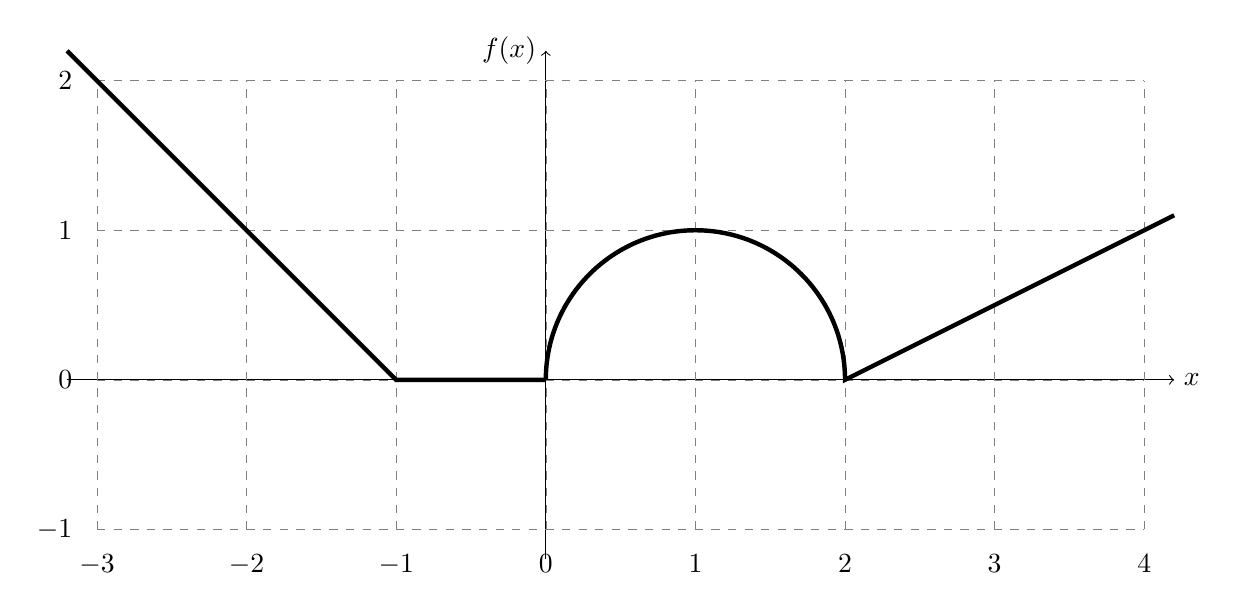
\begin{tikzpicture}[scale=1.9]
\draw[->] (-3.2,0) -- (4.2,0) node[right] {$x$};
\draw[->] (0,-1.2) -- (0,2.2) node[left] {$f(x)$};
\draw[help lines, dashed] (-3,-1) grid (4,2);
\draw[style= ultra thick] (-3.2,2.2) --  (-1,0) -- (0,0);
\draw[style= ultra thick] (0,0) arc (180:0:1) -- (4.2,1.1);
\foreach \x in {-3,-2,-1,0,1,2,3,4}
\draw (\x,-1.1) node[below] {$\x$};
\foreach \y in {-1,0,1,2}
\draw (-3.1,\y) node[left] {$\y$};
\end{tikzpicture}
\end{center}

\bigskip
\begin{enumerate}
\item At what $x$ values, if any, does $f'(x)$ not exist?

\vfill

\item  What is the value of $f'(-2)$?

\vfill

\item  Evaluate $\ds \int_{-1}^{4} f(x)\,dx$.

\vfill

\item  Let $g(x) =\ds \int_1^x f(s)\,ds$.  What is the value of $g(0)$?

\vfill

\item  For $g(x)$ from part \textbf{d.}, what is the value of $g'(4)$.

\vfill
\end{enumerate}


\end{enumerate}
\end{document}
%proto Riemann Sums
\item The graph of the function $\ds f(x)=\sqrt {x^2+3}$ is shown.

\vskip -0.8in
	\begin{enumerate}
\begin{minipage}{0.5\textwidth}
	\item
	On the graph sketch 3 rectangles, using left endpoints, that would be used to
	approximate
	$$\int_1^4 \sqrt{x^2+3}\,dx.$$
	%\vskip 1.in
\end{minipage}
\qquad
\begin{minipage}{0.5\textwidth}
	\vskip 0.5in
	\pgfplotsset{my style/.append style={axis x line=middle, axis y
			line=middle, xlabel={$x$}, ylabel={$y$}}}
	\begin{tikzpicture}
	\begin{axis}[scale=1, my style, xtick={ 0,...,5}, ytick={0,...,6},
	xmin=-.5, xmax=5.5, ymin=-1, ymax=7, minor y tick num=0,
	minor x tick num=0, mark size=5.0pt,
	grid=both, ylabel=$f(x)$,samples=60]
	\addplot[domain=0:5, -, ultra thick] {sqrt(x^2+3};
	\end{axis}
	\end{tikzpicture}
\end{minipage}

\bigskip
\item  Compute the approximation in part {(a)}.  You do not need to simplify, but your answer should be in a form where a calculator
would compute a numerical value.\\
\vfill
\item Is your estimate from part(b) an underestimate or an overestimate? Explain.
\vspace{.5in}
\newpage
\end{enumerate}
